\section{Problema 3 - Biohazard}
\index{Problema 3 - Biohazard}


\subsection{Descripción del problema a resolver}

El problema que trataremos en la presente sección consiste en ubicar en la menor cantidad de camiones posibles una serie de compuestos químicos para su traslado. Cada producto tiene un nivel de peligrosidad con cada uno de los otros. A su vez, los camiones toleran hasta un margen $M$ de peligrosidad acumulada\footnote{La suma de todas las peligrosidades de los productois en su interior tomadas de a pares} en su interior (los camiones son iguales entre si). 

Se nos pide entonces un algoritmo capaz de asociar cada producto a un camión de forma tal de emplear los menos camiones posibles respetando los niveles de tolerancia impuestos. 

Notemos que este problema siempre tiene solución ya que si cada producto se ubica en solitario el traslado será seguro.

Como requerimiento extra tendremos que emplear la técnica algorítmica conocida como \textit{Backtracking} que detallaremos brevemente más adelante.

Veamos algunas instancias de este problema para entender algunos detalles más:

\begin{figure}[H]
\centering
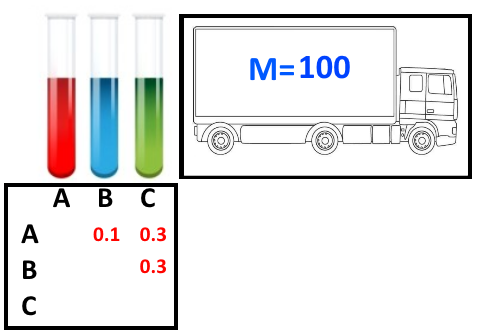
\includegraphics[scale=0.65]{ej3/instancia0.png}
\caption{Instancia con 3 productos y sus peligrosidades. Cada camión tolera hasta 100 de peligrosidad total}
\end{figure}


\begin{figure}[H]
\centering
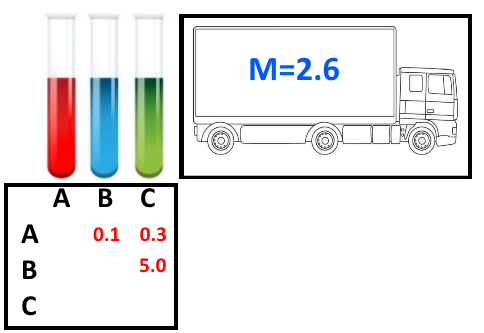
\includegraphics[scale=0.65]{ej3/instancia1.png}
\caption{Instancia con 3 productos y sus peligrosidades. Cada camión tolera hasta 2.6 de peligrosidad total}
\end{figure}

La representación de la entrada que recibiría el algoritmo para esta instancia se ve de la siguiente manera:

\begin{addmargin}[4em]{0em}
\textsf{8 3 0 0 1 1 1 1 0 0} \\
\textsf{0}
\end{addmargin}
\textbf{DESCRIPCIÓN DE LA ENTRADA}

Notemos que el producto A se lleva relativamente bien con el B y el C para los niveles tolerados por los camiones pero que B y C definitivamente no pueden compartir camión. Por este motivo la solución constará de 2 camiones en donde en un camión irá B, en otro C y A en cualquiera de ellos. 

Mientras la solución minimice los camiones, podremos devolver cualquiera de ellas. En particular nuestro algoritmo devuelve: 

\begin{addmargin}[4em]{0em}
\textsf{8 3 0 0 1 1 1 1 0 0} \\
\textsf{0}
\end{addmargin}

\textbf{DESCRIPCIÓN DE LA SALIDA}


\begin{figure}[H]
\centering
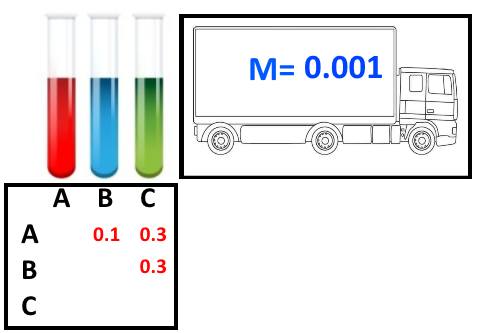
\includegraphics[scale=0.65]{ej3/instancia2.png}
\caption{Instancia con 3 productos y sus peligrosidades. Cada camión tolera hasta 0.0001 de peligrosidad total}
\end{figure}


%
%\subsection{Ideas desarrolladas para la resoluci\'on}
%Para el desarrollo de la resoluci\'on del problema nos basamos primeramente en el dibujo de la figura 1.1: pensamos que tenemos n productos, $p_{1} \dots p_ {n}$. Luego, cada producto $p_{i}$ hay que insertarlo en alg\'un cami\'on $c_{j}$. Como todos los camiones tienen el mismo l\'imite M de biohazard que soportan, es irrelevante en qu\'e n\'umero de cami\'on vamos a introducir cada producto. Lo \'unico que nos va a importar va a ser c\'omo distribuimos los productos de forma relativa entre ellos de tal forma que minimizemos la cantidad de camiones utilizados. Es decir, los camiones son indistinguibles entre s\'i. Con lo cual, como se puede ver en el dibujo, nuestro algoritmo en el paso $i$ prueba recursivamente con todas las combinaciones posibles que se pueden dar tras colocar el producto $p_{i}$ en alguno de los $k$ primeros camiones, donde $k$ es el \'indice del primer cami\'on que estaba  vac\'io antes del comienzo del paso i. Esta poda la nombramos en los comentarios del c\'odigo y la llamamos PODA 1.
%En el ejemplo, colocamos el producto 1 en el cami\'on 1, el 2 en el 1, el 3 en el 2 y el 4 en el 2. Con lo cu\'al, en el paso 5 vamos a probar todas las posibles combinaciones que pueden llegar a derivar de colocar el producto 5 en el cami\'on 1, 2 o 3. No tiene sentido probar qu\'e suceder\'ia colocando el producto 5 en el cami\'on 4 o 5 pues los camiones 3, 4 y 5 son indistinguibles con lo cual alcanza con elegir uno de estos. Nosotros optamos por elegir siempre el de menor \'indice. \\
%
%La otra poda importante que implementamos fue la de que cuando estamos buscando alg\'un cami\'on para colocar el producto $p_{i}$, nos fijamos si la cantidad de camiones ya utilizados en la subsoluci\'on actual (antes de agregar al producto $p_{i}$) es mayor que la mejor soluci\'on obtenida hasta el momento. Si este fuera el caso, entonces no analizamos los casos provenientes de agregar (para la configuraci\'on actual de productos en camiones) los productos $p_{i+1} \dots p_{n}$ porque ya sabemos que la soluci\'on que nos provean va a ser peor que la que ya conseguimos. Esta poda esta nombrada en el c\'odigo y la llamamos PODA 2. \\
%Observaci\'on: como la complejidad del algoritmo de por s\'i es muy grande, optamos por limitar la cantidad de productos que analizamos a 20, ya que para valores un poco m\'as grandes de $n$ sabemos que el algoritmo va a tardar mucho tiempo. \\
%
%\begin{center}
%    \includegraphics [width=20cm]{dibujo1_ej3.png}
%   {Fig. 3.1}
%\end{center}
%
%
%
%Para tener en cuenta, las estructuras de datos importantes de las que hacemos uso son:
%
%\begin{itemize}
%
%\item una matriz de enteros, hazards que dice para cada par de productos, cu\'al es el hazard que generan entre ellos
%\item un entero primerCamionVacio que lleva la cuenta de cu\'al es el \'indice del primer cami\'on vac\'io que en la soluci\'on temporal todav\'ia no usamos.
%\item un entero, mejorHastaAhora, que lleva la cuenta de la m\'inima cantidad de camiones que logramos utilizar para meter los productos hasta el momento
%\item un arreglo de enteros, resTemp, que lleva el resultados temporal (es decir, la data de en qu\'e cami\'on metimos cada uno de los productos considerados hasta el momento)
%\item un vector de enteros, productosEnCamion, que lleva la cuenta de qu\'e productos tenemos metidos en cada cami\'on.  
%\item un vector de enteros, hazardCamion, que lleva la cuenta para cada cami\'on, cu\'al es su hazard total en funci\'on de los productos que hay en \'el (siempre debe ser menor o igual a M)
%\item un arreglo de enteros, hazard2.En la posici\'on $i$ de este arreglo est\'a el hazard que genera el conjunto de productos representados por el entero $i$.
% 
%
%\end{itemize}
%
%
%A continuaci\'on vamos a introducir un pseudoc\'odigo con las ideas b\'asicas que tuvimos en cuenta a la hora de la implementaci\'on: \\
%
%resolver(producto i, resTemp): \\
%
% \hspace{1cm}if (me pase del ultimo producto) terminar \\
% 
% \hspace{2cm} for (camionj in 0 $\dots$ primer camion todav\'ia vac\'io): \\
%	\hspace{3cm} if (se puede agregar el producto i al camion camion camionj):\\
%    	\hspace{4cm} meter producto i en camion camionj, actualizando resTemp \\
%        \hspace{4cm} meter producto productoi en camion camionj \\
%        \hspace{4cm} actualizar el hazard del camion camionj \\
%        \hspace{4cm} if (camionj es el primer camion vacio): \\
%        	\hspace{5cm} actualizo primerCamionVacio \\
%            	
%        \hspace{4cm} if(puede ser mejor soluci\'on): resolver(producto i+1, resTemp) \\
%        
%        \hspace{4cm} if (llegue al \'ultimo producto): \\
%        	\hspace{5cm} if (primerCamionVacio $\leq$ mejorHastaAhora): \\
%            	\hspace{6cm} actualizo mejorHastaAhora = primerCamionVacio \\
%                \hspace{6cm} resultado = resTemp \\
%        \hspace{4cm} saco el producto i del camion camionj \\
%        \hspace{4cm} reestablezco el hazard que le corresponde al camion camionj \\
%        \hspace{4cm} if (camionj era el primer cami\'on todav\'ia vac\'io): \\
%        	\hspace{5cm} actualizo primerCamionVacio \\
%
% \hspace{1cm} terminar \\
% 
%
%
%% ESTARIA BUENO HACER EXPERIMENTOS PODANDO/NO PODANDO PARA VER COMO CAMBIA LA COMPLEJIDAD, MIRANDO GRAFIQUITOS.%
%
%\subsection{Justificaci\'on de complejidad}
%Primero que nada, se ve f\'acilmente que la funci\'on llenarHazards tiene una complejidad temporal de $O(n^{2} 2^{n})$. De esta forma, cada vez que queramos acceder al hazard total de un conjunto de productos vanos a tener acceso en $O(1)$	y no en $O(n)$. Vamos a ver que esta complejidad, necesaria para precalcular resultados que utilizaremos durante el backtracking, es menor que la complejidad del backtracking en s\'i mismo. Esto quiere decir que, esos c\'aclulos previos van a mejorar la los tiempos de ejecuci\'on del algoritmo, por la ganancia en tiempo de acceso al hazard total de un conjunto de productos. \\
%Algo destacable es que con esta implementaci\'on, ganamos complejidad temporal, pero perdemos complejidad espacial(usamos mucho espacio para guardar los hazards generados por todos los posibles subconjuntos de productos).
%
%%OPCION 1
%Para calcular la complejidad temporal de peor caso de nuestro algoritmo de backtracking, vamos a analizar, en funci\'on del para\'ametro de entrada $n$, la cantidad de resultados y sub-resultados intermedios que recorremos para decidir cu\'al es el ordenamiento \'optimo para nuestro problema en cuesti\'on. Como se puede ver, si no hici\'eramos podas, se cumplir\'ia la recurrencia $T(i) = i*T(i-1)$, a partir de la cual sencillamente se puede concluir que $T(n) = O(n!) \in O(n^n)$, por la f\'ormula de Stirling. \\
%
%%OPCION 2
%Sin embargo, con las podas que introdujimos, la complejidad temporal del algoritmo es $3^{n}$ porque en total visitamos $\sum\limits_{i=1}^n {n \choose i}2^{i}$ estados distintos en nuestro algoritmo (la igualdad se deduce de forma directa a partir de la F\'ormula de Binomios de Newton). Es decir, repetimos la funci\'on resolver $n$ veces, y en cada repetici\'on $i$, nos fijamos por cada forma de seleccionar esos $i$ productos de los $n$ que tenemos a disposici\'on, qu\'e suceder\'ia para cada una de esas $2^{i}$ formas de seleccionar dichos $i$ productos. \\
%
%
%
%
%
%
%\newpage
%A continuaci\'on, introducimos la parte m\'as relevante del c\'odigo que implementamos para la resoluci\'on del problema.
%\begin{lstlisting}
%void resolver(int productoi, int &primerCamionVacio, int &mejorHastaAhora, vector<int> &resTemp, vector<int> &res, vector<int> &hazardCamion,
%			  vector<int> &productosEnCamion, int &M, int &n, int hazard2[]) {
%    if(productoi == n) { return; }
%    int primerCamionVacioTemp = primerCamionVacio;
%          for(int camionj=0; camionj<=primerCamionVacioTemp; camionj++) {                
%                pair<bool, int> sePuedeAgregar = nuevoHazard(productoi,camionj,productosEnCamion,M,hazard2);
%                int hazardViejo = hazardCamion[camionj];
%                if(sePuedeAgregar.first) {					
%                    resTemp[productoi] = camionj + 1;
%                    productosEnCamion[camionj] += (1<<productoi)
%                    hazardCamion[camionj] = sePuedeAgregar.second
%                    if(camionj == primerCamionVacioTemp) {
%							primerCamionVacio++; 
%					}					
%                    if(primerCamionVacio <= mejorHastaAhora) {
%						resolver(productoi+1, primerCamionVacio, mejorHastaAhora, resTemp, res, hazardCamion, productosEnCamion, M, n, hazard2);
%                    }
%                    if(productoi + 1 == n) {				
%						  if(primerCamionVacio <= mejorHastaAhora) {													
%								mejorHastaAhora = primerCamionVacio;
%								res = resTemp;
%						  }
%					}
%                    productosEnCamion[camionj] -= (1<<productoi	
%                    hazardCamion[camionj] = hazardViejo;
%					if(camionj == primerCamionVacioTemp) { primerCamionVacio--; }		
%                } 
%          }
%          return;
%}
%\end{lstlisting}
% 
% 
%\subsection{Testeos de complejidad}
% 
% 
%En esta secci\'on, analizamos la i) complejidad del algoritmo sin podas, ii) complejidad del algoritmo con PODA 1, iii) complejidad del algoritmo con PODA 2, iv) complejidad del algoritmo con ambas podas. En el caso en que utilizamos las dos podas, estudiamos qu\'e sucede en los casos peor, promedio y mejor. \\ 
% 
% 
%\subsection{Análisis experimental de podas}
%
%
